\documentclass[nobib]{MSword}
% Class options:
%-------------------------------
% nobib         - skip bibliography code/ don't include bib
% math          - include math packages and useful math commands
% hidelinks     - hide hyperref colored link boxes
% wordlinks     - link color scheme similar to word


% Preamble code:
%%%%%%%%%%%%%%%%%%%%%%%%%%%%%%%%%%%%%%%%
\usepackage[english]{babel}
\usepackage{csquotes}
\usepackage{lipsum}

% % Uncomment using "Ctrl + /" (/ on numpad):
% % Customizing headers and footers:
% \fancypagestyle{custom}{%
%     \fancyhf{}% clears the footer and header
%     % Header:
%     \fancyhead[L]{}
%     \fancyhead[C]{}
%     \fancyhead[R]{}
%     % Footer:
%     \fancyfoot[L]{}
%     \fancyfoot[C]{}
%     \fancyfoot[R]{}
%         % Tips:
%         % ----
%         % L: left, C: center, R: right
%         % O: odd pages, E: even pages
%         % ----
%         % Example: \fancyghead[LO,RE]{Text}
%         % will produce "Text" left in the header
%         % on odd pages and right in the header on even pages.
%     % Rules/ lines:
%     \renewcommand{\headrulewidth}{0.4pt}
%     \renewcommand{\footrulewidth}{2pt}
% }
% % Changing the pagestyle:
% \pagestyle{custom}

%%%%%%%%%%%%%%%%%%%%%%%%%%%%%%%%%%%%%%%%

% Preamble information:
%%%%%%%%%%%%%%%%%%%%%%%%%%%%%%%%%%%%%%%%

\title{Block Diagrams and System Stability}
\author{Dre Mata}
\date{1 March 2023}

%%%%%%%%%%%%%%%%%%%%%%%%%%%%%%%%%%%%%%%%

% The document:
%%%%%%%%%%%%%%%%%%%%%%%%%%%%%%%%%%%%%%%%
\begin{document}

\maketitle
\begin{center}
    Part 1:
\end{center}
The objective of part one is to analyze a block diagram using hand calculations, and then gain a better understanding of tools in python that could help analyze on the computer. The first task of part one is to Type the three give functions in factored form. Their forms follow.

\begin{center}
    $G(s) = (s+9)/(s+2)(s+4)(s-8)$
\end{center}

\begin{center}
    $A(s) = (s+4)/(s+3)(s+1)$
\end{center}

\begin{center}
    $B(s) = (s+12)(s+14)$
\end{center}
The next task was to use the scipy.signal.tf2zpk() function to find zeros and poles of the above functions. For B(s) numpy.root() had to be used since it is not a fraction. The next task was to find the open loop transfer function.

\begin{center}
    $H(s) = Y(s)/X(s) = [1 + (s+12)(s+14)]*(s+4)/(s+2)(s+4)(s-8)$
\end{center}
Looking at the transfer function above it can be said that it will not have a stable response. This is because it will have powers of +alpha when converted to the time domain. The next task was to plot the open loop transfer function. This can be seen in figure one. The plot and shows that the transfer function does not have a stable response, because it exponentially increases to infinity.

\begin{center}
    Part 2:
\end{center}
The objective of part two is to analyze a block diagram using hand calculations, and then gain a better understanding of tools in python that could help analyze on the computer. The first task was to find the closed loop transfer function of the block diagram.

\begin{center}
    $H(s) = Y(s)/X(s) = (s+4)/[1 + (s+12)(s+14)](s+3)(s+1)$
\end{center}
The next step was to use type the transfer fucntion using the scipy.signal.convolve() function and find the zeros and poles using the scipy.signal.tfg2zpk() function. Looking at the closed-loop transfer function it can be seen that the function will have a stable response, because there will be only -alpha powers for e. The next task was to plot the closed-loop transfer function using scipy.signal.step(). This plot can be seen in Figure two. The plot shows that the transfer function will have a stable response, because as time increases the response converges.

\begin{center}
    Questions:
\end{center}
1. In Part 1 Task 5, why does convolving the factored terms using scipy.signal.convolve() result in the expanded form of the numerator and denominator? Would this work with your user-defined convolution function from Lab 3? Why or why not?

This is because a convolution is a type of multiplication expansion. This would work with our user-defined convolution function from lab 3 as well, but the scipy.signal.convolve() is just easier to use.

2. Discuss the difference between the open- and closed-loop systems from Part 1 and Part 2. How does stability differ for each case, and why?

An open loop is the transfer function without the numerator. This is because It can be modeled as separating the feed back loop. The closed-loop system is just the regular box diagram shown in the lab handout. Stability was affected, because for the open loop there would have been a +alpha power for e. This creates an unstable response. The closed loop however had a -alpha power for e, this caused a stable response.

3. What is the difference between scipy.signal.residue() used in Lab 6 and
scipy.signal.tf2zpk() used in this lab?

Scipy.signal.tf2zpk() is meant for transfer functions. scipy.signal.residue is really meant for polynomials divided by polynomials.

4. Is it possible for an open-loop system to be stable? What about for a closed-loop system to be unstable? Explain how or how not for each.

Both of these are questions are possible. All it would depend on for both situations is what makes up each individual function in the box diagram. If the algebra works out that there is only -alpha powers for e it will be stable. That is what will determine stability.


\begin{center}
    Figures
\end{center}

Figure 1:

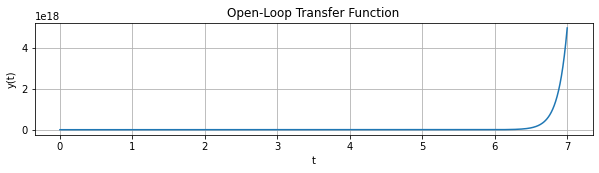
\includegraphics[scale = 0.75]
{txt/Lab7Fig1.png}

Figure 2:

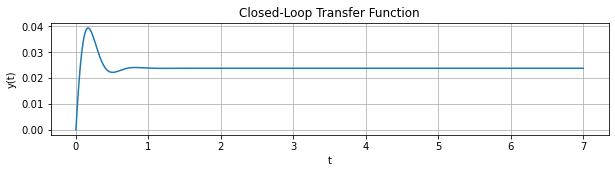
\includegraphics[scale = 0.75]
{txt/Lab7Fig2.png}

\begin{center}
    Conclusion
\end{center}
    This lab helped me gain a better understanding of the tools that I can use in python to analyze box diagrams. The scipy.signal.tf2zpk() function helped show me how easy it is to find roots and poles of transfer functions. This is important, because complex poles tells us that in the time domain the output will be sinusoidal. Also seeing how the transfer functions come out when they are stable vs unstable helped me get a better grasp on what it means for the signs of the exponetial powers.

\end{document}
%%%%%%%%%%%%%%%%%%%%%%%%%%%%%%%%%%%%%%%%

% Copyright Remarks:
%--------------------

% Copyright holder: Vebjørn S. Førde, copyright: CC BY 4.0
% Note: The author of this template is also the copyright holder.

% Below is an explanation of the CC BY 4.0. Additional statements/ 
% clarifications made by the author/copyright holder are marked with *.

% YOU ARE FREE TO:
% Share — copy and redistribute the material in any medium or format
% Adapt — remix, transform, and build upon the material
% for any purpose, even commercially.

% UNDER THE FOLLOWING TERMS:
% Attribution* — You must give appropriate credit, provide a link to the license,
% and indicate if changes were made. You may do so in any reasonable manner, but 
% not in any way that suggests the licensor endorses you or your use.

% *Note: 
% Attribution NOT NEEDED for: 
%       - PDF distibution (like sharing your PDF document)
%       - Use of (dummy)text and images provided in the template (obviously)
%       - Distributing parts of the template, and not the template as a whole
% I am not really concerned with being given credit. As long as you do not 
% claim to have made the template yourself in distributing it further, I have
% no complaints.

% No additional restrictions — You may not apply legal terms or technological 
% measures that legally restrict others from doing anything the license permits.

% NOTICES:
% No warranties are given.

% Disclaimer* (added by copyright holder):
% THE SOFTWARE IS PROVIDED "AS IS", WITHOUT WARRANTY OF ANY KIND, EXPRESS OR
% IMPLIED, INCLUDING BUT NOT LIMITED TO THE WARRANTIES OF MERCHANTABILITY,
% FITNESS FOR A PARTICULAR PURPOSE AND NONINFRINGEMENT. IN NO EVENT SHALL THE
% AUTHORS OR COPYRIGHT HOLDERS BE LIABLE FOR ANY CLAIM, DAMAGES OR OTHER
% LIABILITY, WHETHER IN AN ACTION OF CONTRACT, TORT OR OTHERWISE, ARISING FROM,
% OUT OF OR IN CONNECTION WITH THE SOFTWARE OR THE USE OR OTHER DEALINGS IN THE
% SOFTWARE.

% Read more about CC BY 4.0:
% https://creativecommons.org/licenses/by/4.0/